%-*- coding:utf-8 -*-

\documentclass[10pt,dvipdfmx]{beamer}
\usepackage{tutorial}

\title{計算機実験II (L2) --- 偏微分方程式と多体系の量子力学}
\date{2022/10/28}

\begin{document}

\begin{frame}
  \titlepage
  \tableofcontents
\end{frame}

\begin{frame}[t]{講義日程}
  \begin{itemize}
    % \setlength{\itemsep}{1em}
  \item 全8回 (金曜5限 {\color{red}17:05}-18:35)
    \begin{itemize}
    \item {\color{gray} 10月8日 第1回: 乱択アルゴリズム、モンテカルロ法}
    \item 10月15日 第2回: 多体系の統計力学、マルコフ連鎖モンテカルロ法
    \item 10月22日 第3回
    \item 10月29日 第4回
    \item 11月5日 休講 (もくもく会)
    \item 11月12日 休講 (物理学教室コロキウム)
    \item 11月19日 第5回
    \item 11月26日 休講 (物理学教室コロキウム)
    \item 12月3日 第6回
    \item 12月10日 第7回
    \item 12月17日 休講 (物理学教室コロキウム)
    \item 12月24日 第8回
    \item 1月7日 休講 (もくもく会)
    \item 1月18日(火) 休講 (予備日)
    \end{itemize}
  \end{itemize}
\end{frame}


\section{偏微分方程式の初期値問題}

\begin{frame}[t,fragile]{初期値問題と境界値問題}
  \begin{itemize}
    \setlength{\itemsep}{1em}
  \item 初期値問題
    \begin{itemize}
    \item 微分方程式において、ある1点に関する全ての境界条件(初期値)が与えられているもの
    \item 質点の運動など(時系列の問題)
  \end{itemize}
  \item 境界値問題
    \begin{itemize}
    \item 複数の点に関する境界条件が与えられているもの
    \item 物体のゆがみの計算や静電場の計算など(空間的に解く問題)
  \end{itemize}
  \item 初期値問題は初期値から逐次的に解くことが可能
  \item 境界値問題は初期値問題に比べて計算法が複雑
  \end{itemize}
\end{frame}

\begin{frame}[t]{一次元拡散方程式(放物型)}
  \begin{itemize}
  \item 一次元拡散方程式: $u=u(x,t)$, $q=q(x,t)$
    \[
    \frac{\partial u}{\partial t} - D \frac{\partial^2 u}{\partial x^2} = q
    \]
    \begin{itemize}
    \item 初期条件: $u(x,0) = f(x)$
    \item 境界条件: $u(0,t) = u(1,t) = 0$
    \end{itemize}
  \item 時間$t$と位置$x$に関して離散化
    \begin{align*}
      & u_j^n = u(x_j, t_n) \\
      & q_j^n = q(x_j, t_n) \\
      & t_0 = 0, t_1=\Delta t, t_2=2 \Delta t, \cdots, t_n=n \Delta t, \cdots \\
      & x_0 = 0, x_1=\Delta x, x_2=2 \Delta x, \cdots, x_N=N \Delta x = 1 \qquad (\Delta x = 1/N)
    \end{align*}
  \end{itemize}
\end{frame}

\begin{frame}[t]{有限差分法}
  \begin{itemize}
  \item $t$に関して前進差分を考える
    \[
    \frac{\partial u}{\partial t} \Big|_{(j \Delta x, n \Delta t)} = \frac{u_j^{n+1} - u_j^n}{\Delta t} + {\cal O}(\Delta t)
    \]
  \item $x$に関しては中心差分を考える
    \[
    \frac{\partial^2 u}{\partial x^2} \Big|_{(j \Delta x, n \Delta t)} = \frac{u_{j+1}^{n} - 2 u_{j}^{n} + u_{j-1}^{n}}{\Delta x^2} + {\cal O}(\Delta x^2)
    \]
  \item 拡散方程式に代入して整理すると
    \[
    u_{j}^{n+1} = u_{j}^{n} + r (u_{j+1}^{n} - 2 u_{j}^{n} + u_{j-1}^{n}) + \Delta t q_{j}^{n} \qquad (r = D\frac{\Delta t}{\Delta x^2})
    \]
  \item FTCS (Forward-Time Centered Space)法
  \end{itemize}
\end{frame}

\begin{frame}[t]{FTCS法}
  \begin{itemize}
  \item $O(\Delta t) + O(\Delta x^2)$の陽解法
    \begin{center}
      \resizebox{0.4\textwidth}{!}{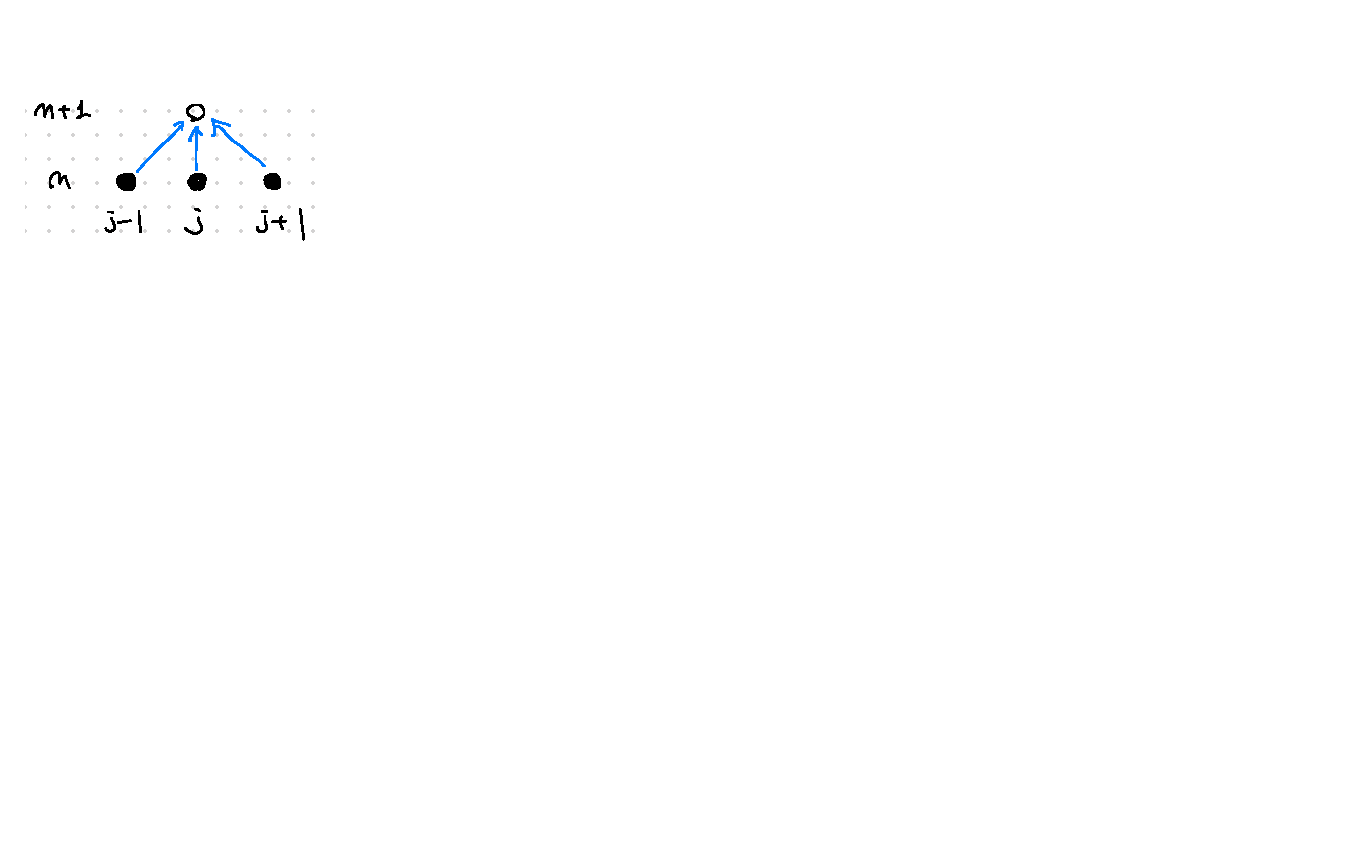
\includegraphics{image/ftcs-1.pdf}}
    \end{center}
  \item 初期条件
    \[
    u_j^0 = f(j\Delta x) \ \ (j=0,1,\cdots,N)
    \]
  \item 境界条件
    \[
    u_0^n = u_N^n = 0 \ \ (n=0,1,2,\cdots)
    \]
  \end{itemize}
\end{frame}

\begin{frame}[t]{有限差分法の安定性}
  \begin{itemize}
  \item (陽的)有限差分法においては、$\Delta t$、$\Delta x$は小さければ小さいほどよいというわけではない
  \item 一次元拡散方程式の場合
    \begin{align*}
      \begin{cases}
        r \le 1/2 & \text{安定} \\
        r > 1/2 & \text{\color{red}不安定}
      \end{cases}
    \end{align*}
  \item $\Delta x$を半分にしたら、$\Delta t$は1/4にしなければならない

    $\Rightarrow$ 計算量は8倍
  \end{itemize}
\end{frame}

\begin{frame}[t]{一次元波動方程式(双極型)}
  \begin{itemize}
  \item 一次元波動方程式
    \[
    \frac{\partial^2 u}{\partial t^2} = c^2 \frac{\partial^2 u}{\partial x^2} \qquad u(x,0)=f(x), \frac{\partial u}{\partial t} (x,0) = g(x)
    \]
  \item $t$に関する中心差分
    \[
    \frac{\partial^2 u}{\partial t^2} \Big|_{(j \Delta x, n \Delta t)} = \frac{u_{j}^{n+1} - 2 u_{j}^{n} + u_{j}^{n-1}}{\Delta t^2} + {\cal O}(\Delta t^2)
    \]
  \item 代入して整理すると
    \[
    u_{j}^{n+1} = 2u_{j}^{n} - u_{j}^{n-1} + \alpha^2 (u_{j+1}^{n} - 2 u_{j}^{n} + u_{j-1}^{n}) \qquad (\alpha = c\frac{\Delta t}{\Delta x})
    \]
  \end{itemize}
\end{frame}

\begin{frame}[t]{波動方程式に対するFTCS法}
  \begin{itemize}
  \item $O(\Delta t^2) + O(\Delta x^2)$の陽解法
    \begin{center}
      \resizebox{0.4\textwidth}{!}{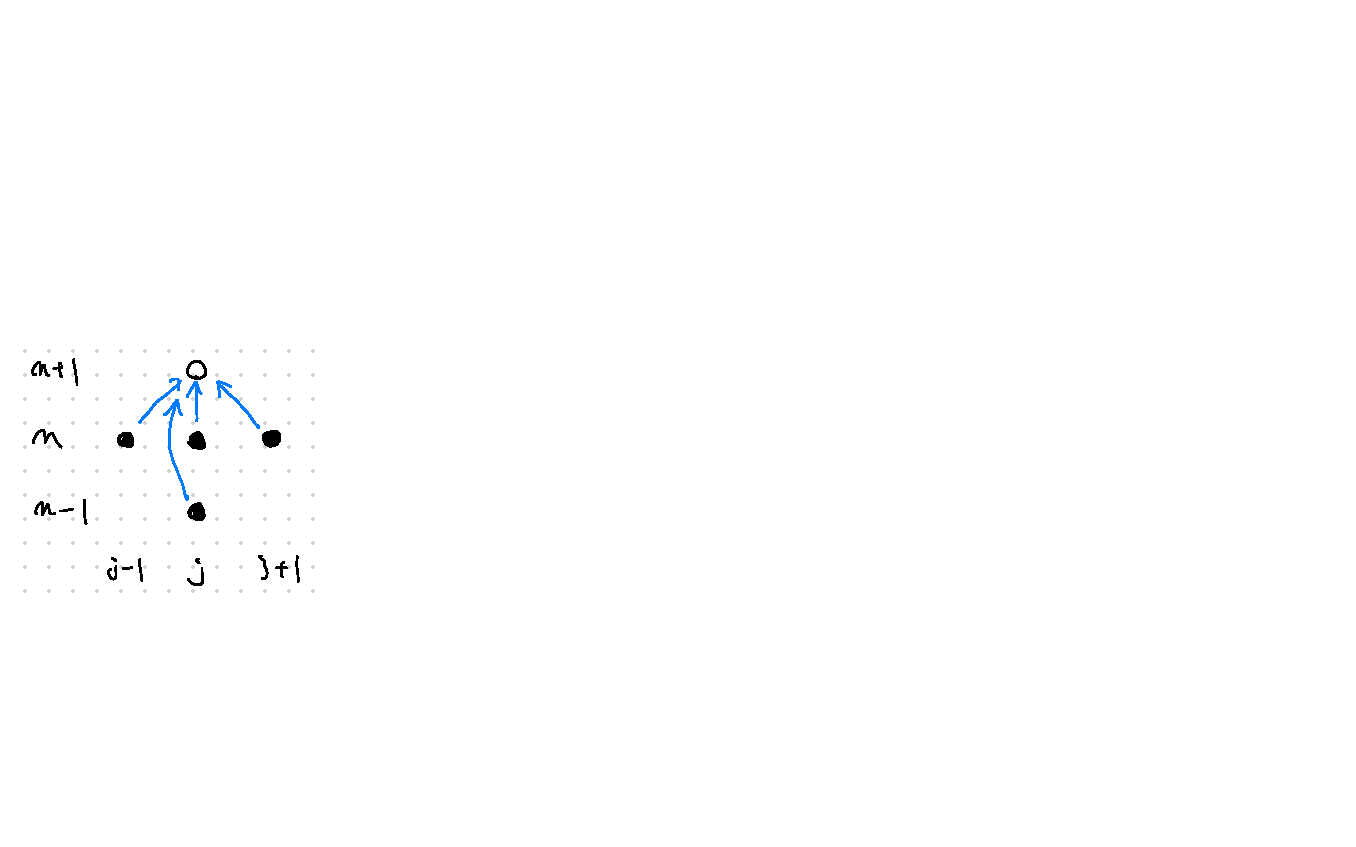
\includegraphics{image/ftcs-2.pdf}}
    \end{center}
  \item 初期条件
    \[
    u_j^0 = f(j\Delta x) \ \ (j=0,1,\cdots,N)
    \]
    初期速度については$n=0$に関する中心差分を考えて
    \[
    \frac{u_j^1 - u_j^{-1}}{2 \Delta t} = g_j \ \ \Rightarrow \ \ u_j^1 = u_j^0 + \Delta t g_j + \frac{\alpha^2}{2} (u_{j+1}^{n} - 2 u_{j}^{n} + u_{j-1}^{n})
    \]
  \end{itemize}
\end{frame}

\begin{frame}[t]{時間に依存するシュレディンガー方程式}
  \begin{itemize}
  \item 時間に依存するシュレディンガー方程式
    \[
    i \hbar \frac{\partial \Psi}{\partial t}(x,t) = H(x,t) \Psi(x,t) = \Big[ - \frac{\hbar^2}{2m} \frac{\partial^2}{\partial x^2} + V(x,t) \Big] \Psi(x,t)
    \]
    \begin{itemize}
    \item 波動関数のノルム $\displaystyle \int | \Psi(x,t) |^2 \, dx$ は保存
    \item $V(x,t)$が時間$t$に依存しない場合、エネルギーの期待値は保存
      \[
      \langle H \rangle = \frac{\displaystyle \int \Psi^* H \Psi \, dx}{\displaystyle \int | \Psi |^2 \, dx}
      \]
    \end{itemize}
  \item 以下では無次元化して$\hbar = m = 1$とおく
  \end{itemize}
\end{frame}

\begin{frame}[t]{時間に依存するシュレディンガー方程式}
  \begin{itemize}
  \item シュレディンガー方程式の形式解 ($V$が時間に依存しない場合)
    \[
    \Psi(x,t) = e^{-i H t} \Psi(x,0)
    \]
  \item $t$に関して前進差分
    \begin{align*}
      e^{-i H t} &= [e^{-i H \Delta t}]^M \approx [1 - i H \Delta t]^M \qquad (\Delta t = t / M) \\
      \Psi^{n+1} &= (1 -  i \Delta t H) \Psi^{n}
    \end{align*}
  \item $H$は対称(エルミート)行列 $\Rightarrow$ 時間発展演算子$e^{-i H \Delta t}$はユニタリー行列
  \item 差分近似$(1 -  i \Delta t H)$はユニタリーではない
    \begin{align*}
      & (e^{-i H \Delta t})^\dagger e^{-i H \Delta t} = e^{i H \Delta t} e^{-i H \Delta t} = 1 \\
      & (1 -  i \Delta t H)^\dagger (1 -  i \Delta t H) = (1 +  i \Delta t H) (1 -  i \Delta t H) = 1 + {\color{red} \Delta t^2 H^2}
    \end{align*}
  \end{itemize}
\end{frame}

\begin{frame}[t]{クランク・ニコルソン法}
  \begin{itemize}
  \item クランク・ニコルソン法
    \[
    \Psi^{n+1} = \frac{1 -  i \frac{\Delta t}{2} H}{1 +  i \frac{\Delta t}{2} H} \Psi^{n}
    \]
  \item (数値精度の範囲で)ユニタリー行列であるので、ノルムは保存
  \item $(1 +  i \frac{\Delta t}{2} H)^{-1}$を掛ける $\Rightarrow$ 連立一次方程式を解く必要がある
    \begin{itemize}
    \item まず、$\Psi = (1 - i \frac{\Delta t}{2} H) \Psi^n$ を計算
    \item 次に、$(1 +  i \frac{\Delta t}{2} H) \Psi^{n+1} = \Psi$ を解く(連立一次方程式)
    \end{itemize}
  \item 陰解法の一種
  \end{itemize}
\end{frame}

\begin{frame}[t]{拡散方程式に対する陰解法}
  \begin{itemize}
  \item 時刻$t$関して後退差分を使う
    \[
    \frac{\partial u}{\partial t} \Big|_{(j \Delta x, n \Delta t)} = \frac{u_j^{n} - u_j^{n-1}}{\Delta t} + {\cal O}(\Delta t)
    \]
  \item $x$に関する中心差分と組み合わせ、$n \rightarrow n+1$と書き直すと
    \[
    u_{j}^{n+1} = u_{j}^{n} + r (u_{j+1}^{n+1} - 2 u_{j}^{n+1} + u_{j-1}^{n+1})
    \]
    $u^{n+1}$が両辺に現れる $\Rightarrow$ 陰解法
  \item $O(\Delta t) + O(\Delta x^2)$
  \item $r$の値によらず{\color{red}常に安定}
  \end{itemize}
\end{frame}

\begin{frame}[t]{拡散方程式に対するクランク・ニコルソン法}
  \begin{itemize}
  \item さらに、時間方向にきざみ幅$\Delta t/2$の中心差分を使うと
    \[
    \frac{\partial u}{\partial t} \Big|_{(j \Delta x, n \Delta t)} = \frac{u_j^{n+\frac{1}{2}} - u_j^{n-\frac{1}{2}}}{\Delta t} + {\cal O}(\Delta t^2)
    \]
  \item $x$に関する中心差分と組み合わせ、$n \rightarrow n+\frac{1}{2}$し、さらに$u_j^{n+\frac{1}{2}}$を$(u_j^{n+1}+u_j^{n})/2$で近似すると
    \[
    u_{j}^{n+1} = u_{j}^{n} + \frac{r}{2} (u_{j+1}^{n+1} - 2 u_{j}^{n+1}  +u_{j-1}^{n+1} + u_{j+1}^{n} - 2 u_{j}^{n} + u_{j-1}^{n})
    \]
    あるいは
    \[
    u_{j}^{n+1} - \frac{r}{2} (u_{j+1}^{n+1} - 2 u_{j}^{n+1} + u_{j-1}^{n+1}) = u_{j}^{n} + \frac{r}{2} (u_{j+1}^{n} - 2 u_{j}^{n} + u_{j-1}^{n})
    \]
    $\Rightarrow$ クランク・ニコルソン法 [$O(\Delta t^2) + O(\Delta x^2)$]
  \end{itemize}
\end{frame}


% \section{対角化 (復習)}
% \begin{frame}[t,fragile]{シュレディンガー方程式の行列表示}
  \begin{itemize}
    %\setlength{\itemsep}{1em}
  \item シュレディンガー方程式
    \[
    [-\frac{d^2}{dx^2}+V(x)]\psi(x) = E \psi(x)
    \]
  \item 連立差分方程式を行列の形で表す($\psi(x_0)=\psi(x_n)=0$)
    \begin{footnotesize}
    \[
    \begin{pmatrix}
      \frac{2}{h^2}+V(x_1) & -\frac{1}{h^2} \\
      -\frac{1}{h^2} & \frac{2}{h^2}+V(x_2) & -\frac{1}{h^2} \\
      & -\frac{1}{h^2} & \frac{2}{h^2}+V(x_3) & -\frac{1}{h^2} \\
      & & \ddots & \ddots \\
      & & & -\frac{1}{h^2} & \frac{2}{h^2}+V(x_{n-1}) \\
    \end{pmatrix}
    \begin{pmatrix}
      \psi(x_1) \\
      \psi(x_2) \\
      \psi(x_3) \\
      \vdots \\
      \psi(x_{n-1}) \\
    \end{pmatrix}
    = \cdots % E
    %% \begin{pmatrix}
    %%   \psi(x_1) \\
    %%   \psi(x_2) \\
    %%   \psi(x_3) \\
    %%   \vdots \\
    %%   \psi(x_{n-1}) \\
    %% \end{pmatrix}
    \]
    \end{footnotesize}
  \item $(n-1) \times (n-1)$の疎行列の固有値問題
    \begin{itemize}
    \item 固有値: 固有エネルギー
    \item 固有ベクトル: 波動関数
    \end{itemize}
  \end{itemize}
\end{frame}

% \begin{frame}[t,fragile]{固体物理・量子統計物理に現れる行列}
  \begin{itemize}
    %\setlength{\itemsep}{1em}
  \item 強束縛近似(tight-binding approx.)のもとでの第二量子化表示
    \[
    H = -t \sum_{\langle i,j \rangle \sigma} (c_{i,\sigma}^\dagger c_{j,\sigma} + h.c.) + \text{(相互作用)}
    \]
  \item 局所スピン模型(ハイゼンベルグ模型)
    \[
    H = -J\sum_{\langle i,j \rangle} S_i \cdot S_j
    = -J\sum_{\langle i,j \rangle} [S_i^z S_j^z +\frac{1}{2} (S_i^+ S_j^- + S_i^- S_j^+) ]
    \]
  \item 格子点の数を$n$とすると、ハミルトニアンはそれぞれ$4^n \times 4^n$、$2^n \times 2^n$の(疎)行列で表される。
  \item $n$が大きくなると、行列の次元は指数関数的に増加
  \item 量子多体系に共通する困難
  \end{itemize}
\end{frame}

% \begin{frame}[t,fragile]{行列の数値対角化}
  \begin{itemize}
    %\setlength{\itemsep}{1em}
  \item 一般的に次元が5以上の行列の固有値は、あらかじめ定まる有限回の手続きでは求まらない
    \begin{itemize}
    \item 必ず何らかの反復法(+収束判定)が必要となる
    \end{itemize}
  \item 密行列向きの方法
    \begin{itemize}
    \item Jacobi法
    \item Givens変換・Householder法(三重対角化) + QR法など
    \end{itemize}
  \item 疎行列向きの方法
    \begin{itemize}
    \item べき乗法
    \item Lanczos法(三重対角化) + QR法など
    \end{itemize}
  \item 固有ベクトル
    \begin{itemize}
    \item QR法で求めたものを逆変換
    \item 逆反復法で精度改善
    \end{itemize}
  \end{itemize}
\end{frame}


\section{横磁場イジング模型}

\begin{frame}[t,fragile]{横磁場イジング模型}
  \begin{itemize}
    %\setlength{\itemsep}{1em}
  \item ハミルトニアン($2^N \times 2^N$行列)
    \[
      H = H_z + H_x = - J \sum_{\langle i,j \rangle} \sigma_i^z \sigma_j^z - h \sum_i \sigma_i^z - \Gamma \sum_i \sigma_i^x
    \]
  \item $\sigma_i^x$、$\sigma_i^z$: パウリ行列($2 \times 2$行列)
    \begin{align*}
      \big(\sigma_i^z\big)^2 &= \big(\sigma_i^x\big)^2 = I \\
      [ \sigma_i^z, \sigma_i^x ] &\ne 0
    \end{align*}
  \item $J$: スピン間の相互作用($J>0$: 強磁性、$J<0$: 反強磁性)
  \item $h$: 縦磁場(準位間のエネルギー差$=2h$)
  \item $\Gamma$: 横磁場(トンネリング)
  \item 以降、$\sigma_i^z$を対角化する基底($|\!\uparrow\rangle_i$, $|\!\downarrow\rangle_i$)で考える
  \end{itemize}
\end{frame}

\begin{frame}[t,fragile]{横磁場イジング模型}
  \begin{itemize}
    %\setlength{\itemsep}{1em}
  \item 2サイト系
    \[
      H = -J \sigma_1^z \sigma_2^z - h (\sigma_1^z + \sigma_2^z) - \Gamma (\sigma_1^x + \sigma_2^x)
    \]
  \item 行列要素
    \begin{align*}
      \langle \uparrow \uparrow \!| H |\! \uparrow \uparrow \rangle &= -J - 2h \\
      \langle \uparrow \uparrow \!| H |\! \uparrow \downarrow \rangle &= -\Gamma \\
      \langle \uparrow \uparrow \!| H |\! \downarrow \downarrow \rangle &= 0 \\
      &\vdots
    \end{align*}
  \end{itemize}
\end{frame}

\begin{frame}[t,fragile]{量子相転移}
  \begin{itemize}
    %\setlength{\itemsep}{1em}
  \item $h=0$の場合
    \begin{itemize}
    \item $\Gamma \rightarrow 0$: $|\!\uparrow\uparrow\cdots\uparrow\rangle$、あるいは$|\!\downarrow\downarrow\cdots\downarrow\rangle$が基底状態(二重縮退)
    \item $J \rightarrow 0$: $\sigma_i^x$の固有状態($|\!\uparrow\rangle_i + |\!\downarrow\rangle_i$)の積が基底状態(全ての状態の重ね合わせ)
    \end{itemize}
  \item 一次元系
    \[
      H = - J \sum_{i} \sigma_i^z \sigma_{i+1}^z - \Gamma \sum_i \sigma_i^x
    \]
    $\Gamma = J$で量子相転移(熱ゆらぎではなく量子ゆらぎによる相転移)  
  \end{itemize}
\end{frame}


\section{多体量子系の時間発展}

\begin{frame}[t,fragile]{横磁場イジング模型の時間発展}
  \begin{itemize}
    %\setlength{\itemsep}{1em}
  \item 時間依存シュレディンガー方程式の形式解
    \[
    \Psi(t) = e^{-iHt} \Psi(0)
    \]
    \begin{itemize}
    \item 有限差分法、クランク・ニコルソン法
    \end{itemize}
  \item 鈴木・トロッター分解 ($\Delta t = t / M$)
    \begin{align*}
      e^{-iHt} &= \big[ e^{-iH\Delta t} \big]^M \approx \big[ e^{-iH_z\Delta t} e^{-iH_x\Delta t} \big]^M \\
      &= \big[ e^{i\Delta t J \sum_{\langle i,j \rangle} \sigma_i^z \sigma_j^z} e^{i\Gamma \sigma_1^x\Delta t} e^{i\Gamma \sigma_2^x\Delta t} \cdots e^{i\Gamma \sigma_N^x\Delta t} \big]^M
    \end{align*}
    (さらに$e^{-iH\Delta t} \approx e^{-iH_z\Delta t/2} e^{-iH_x\Delta t} e^{-iH_z\Delta t/2}$と対称に分解すると近似の次数が上がる)
  \item $[\sigma_i^x]^2 = I$より
    \[
    e^{i\Gamma \sigma_i^x\Delta t} = \cos (\Gamma\Delta t) + i \sigma_i^x \sin (\Gamma\Delta t)
    \]
  \end{itemize}
\end{frame}

\begin{frame}[t,fragile]{量子アニーリング}
  \begin{itemize}
    %\setlength{\itemsep}{1em}
  \item 離散最適化問題
    \[
    H = -J \sum_{i<j} \epsilon_{ij} \sigma_i^z \sigma_j^z
    \]
    の基底状態配位と基底状態エネルギーを求めたい
    \begin{center}
      \resizebox{0.6\textwidth}{!}{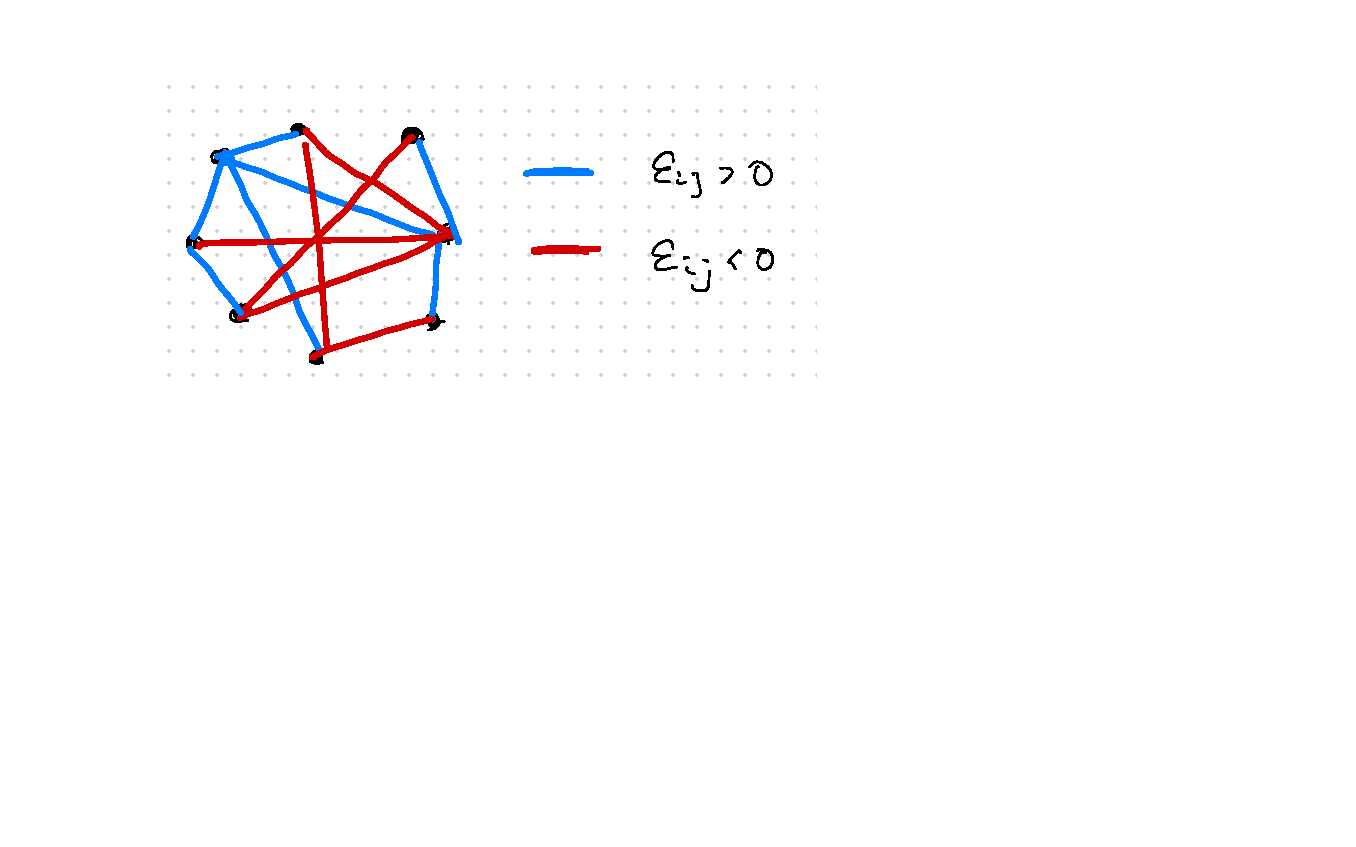
\includegraphics{image/spinglass.pdf}}
    \end{center}
  \end{itemize}
\end{frame}

\begin{frame}[t,fragile]{量子アニーリング}
  \begin{itemize}
    %\setlength{\itemsep}{1em}
  \item 横磁場を導入
    \[
    H = -J \sum_{i<j} \epsilon_{ij} \sigma_i^z \sigma_j^z - \Gamma \sum_i \sigma_i^x
    \]
  \item 古典極限 ($J=1$, $\Gamma=0$)
    \begin{itemize}
    \item 求めたい基底状態
    \end{itemize}
  \item 量子極限 ($J=0$, $\Gamma=1$)
    \begin{itemize}
    \item $2^N$個の全ての状態の重ね合わせ
    \end{itemize}
  \item 量子アニーリング
    \begin{itemize}
    \item $J+\Gamma=1$を保ったままで、$\Gamma=1$から$\Gamma=0$まで「ゆっくり」と減少させながら時間発展させる
      \[
      J = 1-\Gamma = t/T \qquad (0 \le t \le T)
      \]
    \item $T \rightarrow \infty$の極限で確率1で基底状態に収束
    \end{itemize}
  \end{itemize}
\end{frame}


\section{量子コンピュータ}

\begin{frame}[t,fragile]{量子コンピュータと量子ゲート}
  \begin{itemize}
    %\setlength{\itemsep}{1em}
  \item (ゲート型)量子コンピュータ

    $N$量子ビットに対して、量子ゲートにより状態を操作

    \begin{itemize}
    \item 「量子ビット」= 2準位系($S=1/2$スピン) \ $|0\rangle=|\!\uparrow\rangle, |1\rangle=|\!\downarrow\rangle$
    \item 「量子ゲート」= 少数量子ビットに対するユニタリ変換
    \end{itemize}
  \item 1量子ビットゲート
    \begin{itemize}
    \item Xゲート(量子NOT)
      \[
      X = \begin{pmatrix} 0 & 1 \\ 1 & 0 \end{pmatrix} = \sigma^x
      \]
    \item Rzゲート($z$軸まわりの回転)
      \[
      Rz(\theta) = \begin{pmatrix} e^{-i\theta/2} & 0 \\ 0 & e^{i\theta/2} \end{pmatrix} = e^{-i\theta\sigma^z/2}
      \]
    \item アダマールゲート
      \[
      H = \frac{1}{\sqrt{2}} \begin{pmatrix} 1 & 1 \\ 1 & -1 \end{pmatrix} = \frac{1}{\sqrt{2}} (\sigma^x + \sigma^z)
      \]
    \end{itemize}
  \end{itemize}
\end{frame}

\begin{frame}[t,fragile]{量子ビットゲート}
  \begin{itemize}
    %\setlength{\itemsep}{1em}
  \item 2量子ビットゲート
    \begin{itemize}
    \item CXゲート(制御NOT)
      \[
      CX = \begin{pmatrix} 1 & 0 & 0 & 0 \\ 0 & 1 & 0 & 0 \\ 0 & 0 & 0 & 1 \\ 0 & 0 & 1 & 0 \end{pmatrix}
      \]
    \end{itemize}
  \item 3量子ビットゲート
    \begin{itemize}
    \item CCXゲート(トフォリゲート)
      \[
      CCX = \begin{pmatrix}
        1 & 0 & 0 & 0 & 0 & 0 & 0 & 0 \\
        0 & 1 & 0 & 0 & 0 & 0 & 0 & 0 \\
        0 & 0 & 1 & 0 & 0 & 0 & 0 & 0 \\
        0 & 0 & 0 & 1 & 0 & 0 & 0 & 0 \\
        0 & 0 & 0 & 0 & 1 & 0 & 0 & 0 \\
        0 & 0 & 0 & 0 & 0 & 1 & 0 & 0 \\
        0 & 0 & 0 & 0 & 0 & 0 & 0 & 1 \\
        0 & 0 & 0 & 0 & 0 & 0 & 1 & 0 \end{pmatrix}
      \]
    \end{itemize}
  \end{itemize}
\end{frame}

\begin{frame}[t,fragile]{量子加算器}
  \begin{itemize}
    %\setlength{\itemsep}{1em}
  \item 1量子ビットの加算 $\Rightarrow$ CCXゲートとCXゲートで実現できる
    \begin{center}
      \resizebox{0.5\textwidth}{!}{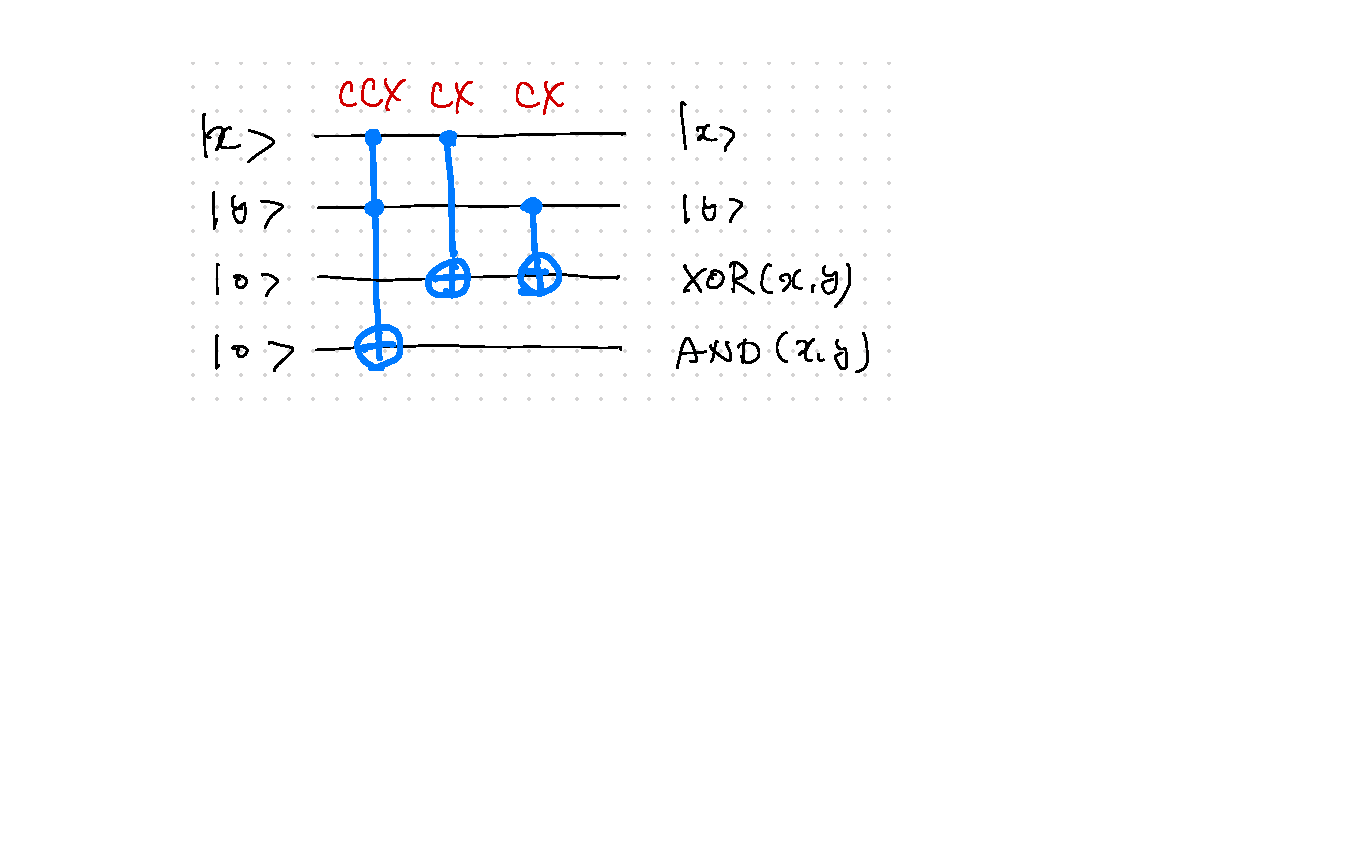
\includegraphics{image/adder1.pdf}}
    \end{center}
  \item CCXゲートは、Hゲート、Rzゲート、CXゲートの組み合わせで表現できる
  \item 任意の量子回路は、Hゲート、Rzゲート、CXゲートの組み合わせで表現できる (万能量子ゲート)
  \end{itemize}
\end{frame}

\begin{frame}[t,fragile]{量子加算器}
  \begin{itemize}
    %\setlength{\itemsep}{1em}
  \item 3量子ビット加算器
    \begin{center}
      \resizebox{0.6\textwidth}{!}{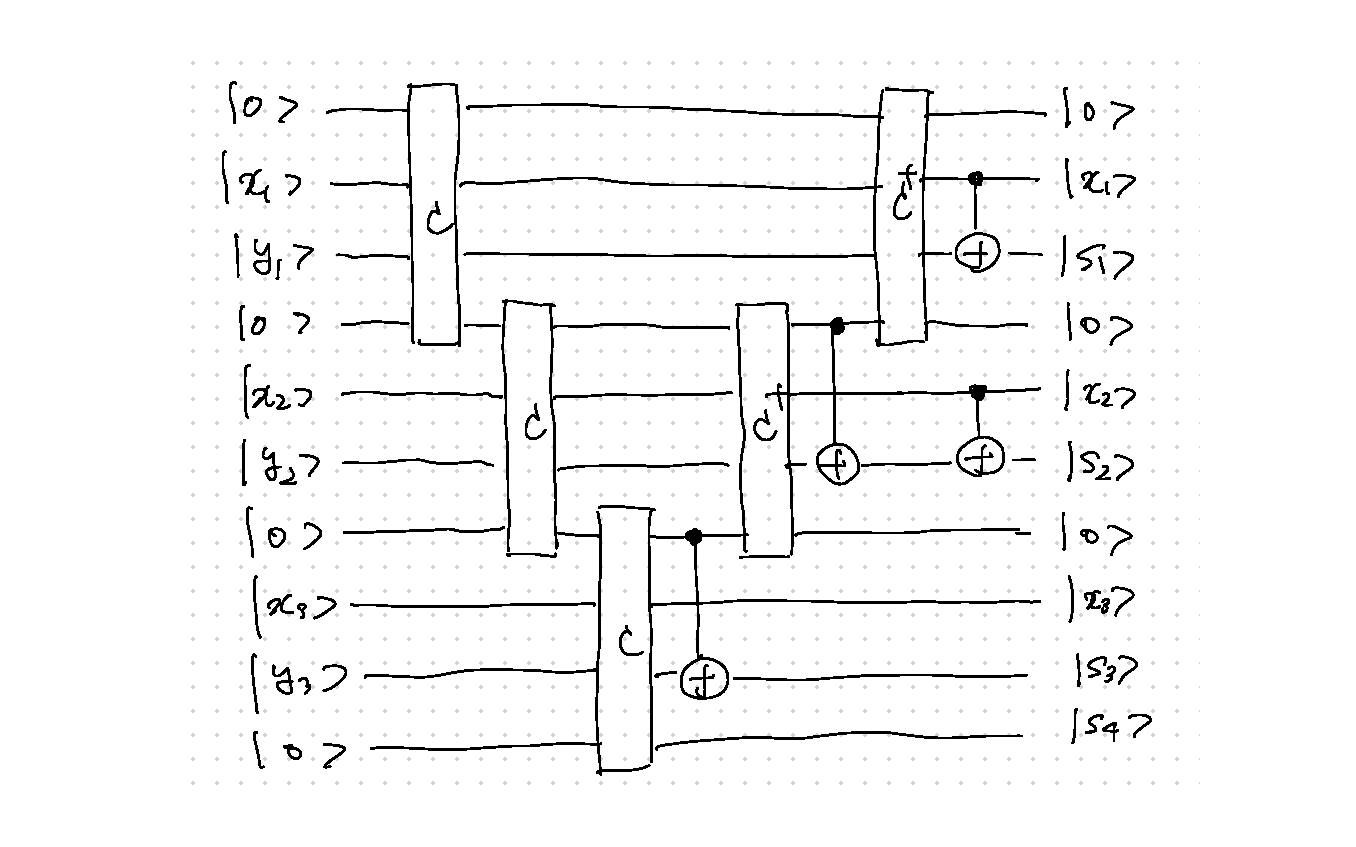
\includegraphics{image/adder3.pdf}}
      \resizebox{0.35\textwidth}{!}{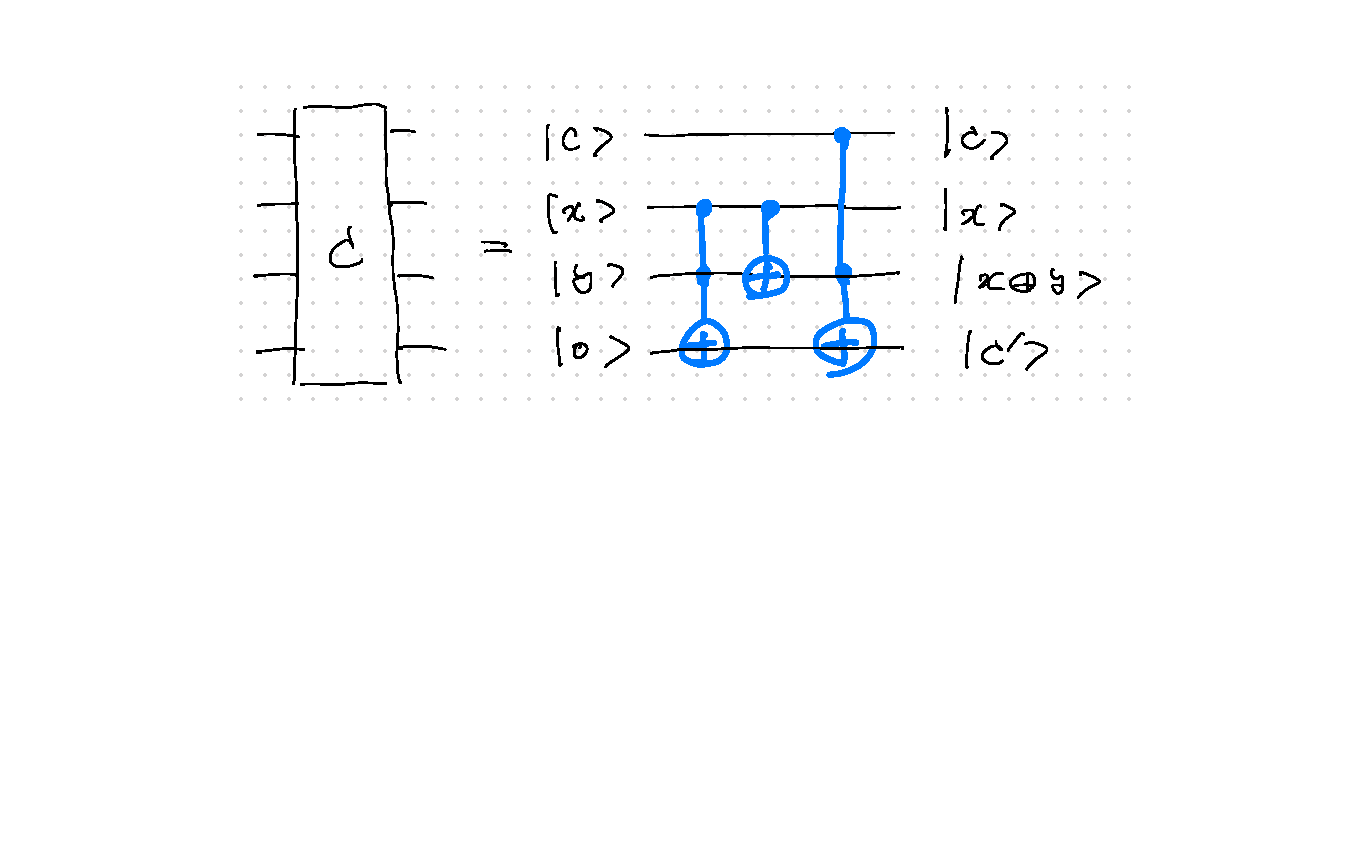
\includegraphics{image/adder2.pdf}}
    \end{center}
  \end{itemize}
\end{frame}


\end{document}
